\chapter{Проектирование интерфейса}
	\section{Целевая аудитория}
		Данная программа разрабатывается для следующих категорий пользователей:
		\begin{itemize}
			\item Архитекторы программных комплексов, основанных на модели ДВС.
			\item Архитекторов ЭВМ, функционирующих по модели ДВС.
		\end{itemize}
	
		\medskip

		Требования к пользователю:
		\begin{enumerate}
			\item Понимание модели ДВС.
			\item Наличие элементарных навыков работы с приложениями.
		\end{enumerate}
	
	\section{Целевые функциональные характеристики}
		Программа решает следующие задачи:
		\begin{itemize}
			\item Редоктирование структуры ДВС.
			\item Моделирование процесса в ДВС
		\end{itemize}
	
	\section{Концептуальная модель}
		\subsection{Структура данных}
			Каждая ДВС характеризуется структурой, изображённой на рис. \ref{fig:dcn-data}
			\begin{figure}[th]
				\centering
				\includegraphics[width=\linewidth]{images/DCN-data}
				\caption{Структура данных}
				\label{fig:dcn-data}
			\end{figure}
		
		\subsection{Технологическая цепочка и cтруктура инструментов}
			На рис. \ref{fig:dcn-tech} представлена технологическая цепочка и список инструментов для реализации того или иного вида деятельности.
			\begin{figure}[th]
				\centering
				\includegraphics[width=\linewidth]{images/dcn-tech}
				\caption{Технологическая цепочка и список инструментов}
				\label{fig:dcn-tech}
			\end{figure}
		
		\FloatBarrier
		\clearpage
		\subsection{Перцептивная модель}
		
			\begin{figure}[th]
				\centering
				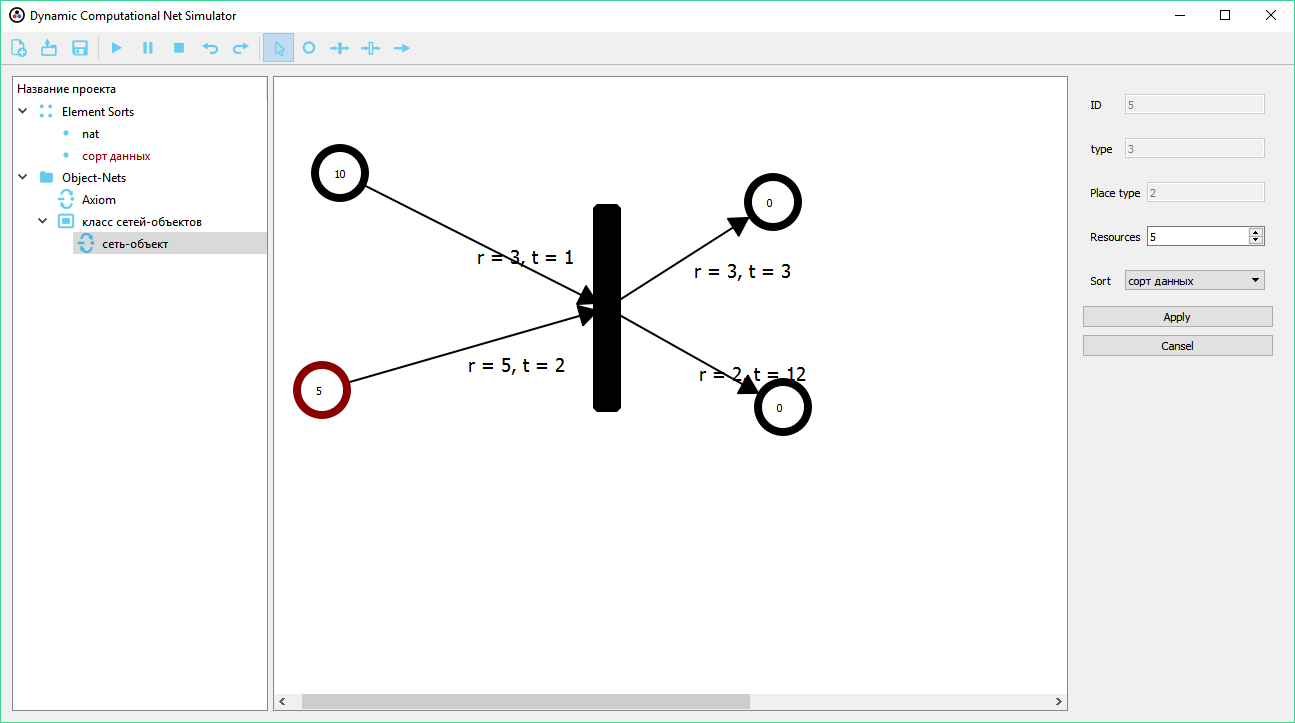
\includegraphics[width=\linewidth]{images/percept}
				\caption{Перцептивная модель}
				\label{fig:percept}
			\end{figure}
